%% 
%% Copyright 2007-2020 Elsevier Ltd
%% 
%% This file is part of the 'Elsarticle Bundle'.
%% ---------------------------------------------
%% 
%% It may be distributed under the conditions of the LaTeX Project Public
%% License, either version 1.2 of this license or (at your option) any
%% later version.  The latest version of this license is in
%%    http://www.latex-project.org/lppl.txt
%% and version 1.2 or later is part of all distributions of LaTeX
%% version 1999/12/01 or later.
%% 
%% The list of all files belonging to the 'Elsarticle Bundle' is
%% given in the file `manifest.txt'.
%% 
%% Template article for Elsevier's document class `elsarticle'
%% with harvard style bibliographic references

%\documentclass[preprint,12pt,authoryear]{elsarticle}

%% Use the option review to obtain double line spacing
%% \documentclass[authoryear,preprint,review,12pt]{elsarticle}

%% Use the options 1p,twocolumn; 3p; 3p,twocolumn; 5p; or 5p,twocolumn
%% for a journal layout:
%% \documentclass[final,1p,times,authoryear]{elsarticle}
%% \documentclass[final,1p,times,twocolumn,authoryear]{elsarticle}
%% \documentclass[final,3p,times,authoryear]{elsarticle}
%% \documentclass[final,3p,times,twocolumn,authoryear]{elsarticle}
%% \documentclass[final,5p,times,authoryear]{elsarticle}
 \documentclass[final,5p,times,twocolumn,authoryear]{elsarticle}

%% For including figures, graphicx.sty has been loaded in
%% elsarticle.cls. If you prefer to use the old commands
%% please give \usepackage{epsfig}

%% The amssymb package provides various useful mathematical symbols
\usepackage{amssymb}
\usepackage{lipsum}
%% The amsthm package provides extended theorem environments
%% \usepackage{amsthm}

%% The lineno packages adds line numbers. Start line numbering with
%% \begin{linenumbers}, end it with \end{linenumbers}. Or switch it on
%% for the whole article with \linenumbers.
%% \usepackage{lineno}

%% You might want to define your own abbreviated commands for common used terms, e.g.:
\newcommand{\kms}{km\,s$^{-1}$}
\newcommand{\msun}{$M_\odot}

\journal{Results in Physics}


\begin{document}

\begin{frontmatter}

%% Title, authors and addresses

%% use the tnoteref command within \title for footnotes;
%% use the tnotetext command for theassociated footnote;
%% use the fnref command within \author or \affiliation for footnotes;
%% use the fntext command for theassociated footnote;
%% use the corref command within \author for corresponding author footnotes;
%% use the cortext command for theassociated footnote;
%% use the ead command for the email address,
%% and the form \ead[url] for the home page:
%% \title{Title\tnoteref{label1}}
%% \tnotetext[label1]{}z
%% \author{Name\corref{cor1}\fnref{label2}}
%% \ead{email address}
%% \ead[url]{home page}
%% \fntext[label2]{}
%% \cortext[cor1]{}
%% \affiliation{organization={},
%%            addressline={}, 
%%            city={},
%%            postcode={}, 
%%            state={},
%%            country={}}
%% \fntext[label3]{}

\title{A Game Theory Simulation on the Battle of Gettysburg using Agent-Based-Modeling}
%% use optional labels to link authors explicitly to addresses:
%% \author[label1,label2]{}
%% \affiliation[label1]{organization={},
%%             addressline={},
%%             city={},
%%             postcode={},
%%             state={},
%%             country={}}
%%
%% \affiliation[label2]{organization={},
%%             addressline={},
%%             city={},
%%             postcode={},
%%             state={},
%%             country={}}

\author{Rubén Hernández O'kelly}
\affiliation{organization={Institute for Computing in Research},
            city={Santa Fe}, 
            state={NM},
            postcode={2023}}

\begin{abstract}
%% Text of abstract
This study employs agent-based modeling and game theory to reexamine the Battle of Gettysburg, a pivotal conflict during the American Civil War. By simulating the battle with agents representing Union and Confederate forces, we investigate the impact of strategic decisions on the battle's outcome. Leveraging game theory principles, the simulation enables agents to adapt their actions based on interactions and environmental factors, shedding light on the complex decision-making dynamics faced by historical generals. The comparison between the simulation and actual historical events reveals insights into the Union's potential strategic advantages and opportunities for improved decision-making.

\end{abstract}

%%Graphical abstract
%\begin{graphicalabstract}
%\includegraphics{grabs}
%\end{graphicalabstract}

%%Research highlights
%\begin{highlights}
%\item Research highlight 1
%\item Research highlight 2
%\end{highlights}

\begin{keyword}
%% keywords here, in the form: keyword \sep keyword, up to a maximum of 6 keywords
Game Theory \sep Agent-based modeling \sep Simulation \sep Gettysburg

%% PACS codes here, in the form: \PACS code \sep code

%% MSC codes here, in the form: \MSC code \sep code
%% or \MSC[2008] code \sep code (2000 is the default)

\end{keyword}


\end{frontmatter}

%\tableofcontents

%% \linenumbers

%% main text

\section{Introduction}
\label{introduction}

“Let your plans be dark and impenetrable as night, and when you move, fall like a thunderbolt.”
― Sun Tzu, The Art of War. Sun Tzu's quote epitomizes the significance of secrecy and surprise in warfare. In the context of the Battle of Gettysburg and the project's exploration of game theory and agent-based modeling, it emphasizes the importance of uncertainty and adaptive decision-making by the generals. Employing this strategic philosophy, simulated agents in agent-based modeling can replicate the challenges faced by real generals, allowing for a deeper understanding of the battle's complex dynamics.

\section{Scenario and Methodology}
%%\label{}
%%\subsection{Backgrounds}

The Battle of Gettysburg, fought from July 1 to July 3, 1863, during the American Civil War, was a pivotal and bloody conflict between the Union Army of the Potomac, commanded by General George G. Meade, and the Confederate Army of Northern Virginia, led by General Robert E. Lee. It took place in the small town of Gettysburg, Pennsylvania, and is often considered the turning point of the Civil War. The battle was a result of Lee's second invasion of the North and his attempt to gain a strategic advantage by taking the war to Union territory. The three-day battle saw intense fighting and heavy casualties on both sides, with approximately 51,000 soldiers killed, wounded, or missing. The Union emerged victorious, and Lee's Confederate forces were forced to retreat back to Virginia, effectively ending the South's hopes for a successful invasion of the North.

The Battle of Gettysburg is renowned for its significance in the Civil War's outcome and its impact on American history. The Union victory boosted Northern morale and solidified President Abraham Lincoln's resolve to issue the Emancipation Proclamation later that year, declaring the freedom of all slaves in Confederate-held territories. Furthermore, the battle prompted Lee to abandon future offensives in the North, shifting the focus of the war to Virginia and eventually leading to the Union's triumph.

Game theory is a branch of mathematics and economics that deals with strategic interactions among multiple decision-makers (players) who aim to maximize their utility or payoff (rewards). It provides a formal framework to analyze and predict how individuals or organizations make decisions in competitive situations. Developed in the mid-20th century, game theory has found applications in various fields, including economics, political science, biology, and computer science. The central concept in game theory is the "game," which consists of players, strategies, and payoffs. Different games, such as Prisoner's Dilemma, Battle of the Sexes, and Chicken, present various scenarios of conflict, cooperation, and decision-making, offering valuable insights into real-world situations.

Agent-Based Modeling (ABM) is a computational modeling technique used to simulate the behavior and interactions of individual agents to understand complex systems' emergent properties. In ABM, agents are autonomous entities that follow predefined rules and adapt their behavior based on their local environment and interactions with other agents. The model's dynamics emerge from the collective behavior of these agents, allowing researchers to observe and analyze the system's macro-level patterns and outcomes. ABM has gained popularity across various domains, including sociology, ecology, economics, and epidemiology, as it provides a powerful tool to study systems that involve numerous autonomous agents and complex interactions. ABM allows researchers to explore "what-if" scenarios, test hypotheses, and gain insights into the system's behavior that may not be apparent through traditional analytical methods.

\section{Methods}
%%\label{}
The simulation results will be compared to the historical outcome of the Battle of Gettysburg to identify effective strategies that the Union could have employed. By applying game theory principles and agent-based modeling, we hope to gain valuable insights into the decision-making dynamics of this critical historical event. 

To conduct the agent-based simulation, we developed a Python program that models the Battle of Gettysburg using game theory principles. The simulation involves two teams, the Union and the Confederacy, each represented by agents with unique characteristics such as health, attack range, and attack strength. The agents follow predefined rules and adapt their actions based on their local environment and interactions with other agents. In the simulation, the number of agents per team has been calculated to be historically accurate while also keeping within program limitations.

The simulation progresses through a series of steps, with each step representing a moment in the battle. At each step, the agents make decisions on whether to attack enemy agents within their attack range or to retreat to a common point for regrouping. The agents' strategies are based on the principles of game theory, seeking to maximize their utility (in this case, winning the battle) while anticipating the opponents' actions.

The program is conducted in such a way that the agents are arranged by formations which resemble those used in the actual battle:

\begin{figure}[!ht]
  \centering
      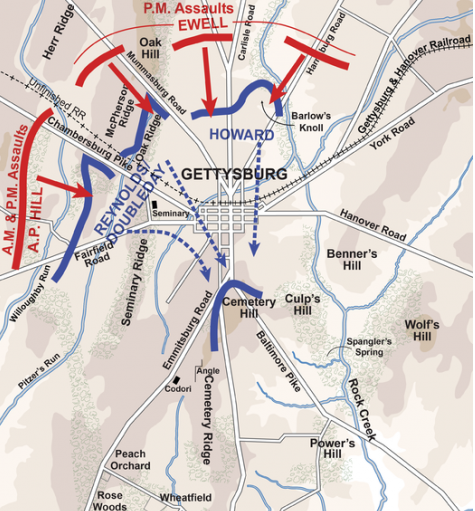
\includegraphics[width=6cm]{Gettysburg_map.png}
      \caption{The map of the Battle of Gettysburg}
      \label{fig:Map}
  \centering
\end{figure}

\begin{figure}[!ht]
  \centering
      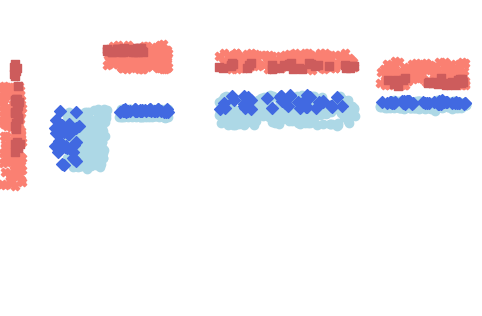
\includegraphics[width=6cm]{sim_gett_map.png}
      \caption{A simulated map of the Battle of Gettysburg}
      \label{fig:Map}
  \centering
\end{figure}

In this simulation, the Red Team are representing the Confederate army at Gettysburg, while the blue agents represent the Union army. The simulation program encompasses several crucial parameters that dictate the dynamics of the Battle of Gettysburg reenactment. The number of agents per team has been meticulously designed to mirror historical records, with a calculated allocation of soldiers and cavalry for both Union and Confederate forces. For instance, the Union's numerical superiority is represented through a larger contingent of soldiers and cavalry units, accurately reflecting the historical troop composition. Moreover, the simulation incorporates a dynamic losing percentage threshold that triggers victory conditions for one side. When either the Union or Confederate forces retain less than a predetermined percentage of their initial strength, the opposing team is declared the victor. This threshold, carefully calibrated based on historical outcomes, introduces a sense of urgency and realism to the simulation, encouraging players to make strategic decisions that align with historical context. Additionally, other parameters such as attack range, attack strength, and retreat strategies are thoughtfully incorporated, enabling agents to execute tactical maneuvers and replicate the complexity of the actual battle. By fine-tuning these parameters, the simulation not only captures historical authenticity but also facilitates an in-depth exploration of the battle's various scenarios and outcomes.

Upon completion of the simulation, we compare the results with the historical outcome of the Battle of Gettysburg. We evaluate the effectiveness of different strategies employed by the Union agents and identify potential improvements in their decision-making. The findings shed light on the significance of adaptive decision-making and the impact of uncertainty on battle outcomes.

The agent-based simulation of the Battle of Gettysburg is conducted using principles derived from Game Theory, where simulated agents representing Union and Confederate forces make strategic decisions based on interactions with other agents and the battlefield environment. By employing Game Theory as the foundation, the simulation aims to recreate the challenges faced by the real generals during the historic battle and uncover the best possible actions that the Union could have taken.

During the simulation, each agent represents a unit in the army, with distinct attributes such as position, health, attack range, and attack strength. The agents utilize the principles of Game Theory to determine their actions, choosing between attacking an enemy agent or retreating to a common point with fellow teammates. The simulation progresses through a series of time steps, and at each step, agents interact with their surroundings and adapt their strategies based on the observed outcomes.

To enhance the realism of the simulation, the agent-based model also introduces stochastic fictitious play, a variant of the fictitious play algorithm in game theory. Stochastic fictitious play adds an element of randomness to the agents' decisions, making their strategies more robust in the face of uncertainty. As the simulation unfolds, the agents update their beliefs about their opponents' strategies and adjust their own actions accordingly, converging towards optimal responses to the mixed strategies of their adversaries. This allows the simulation to capture the dynamic and evolving nature of the battlefield, where unexpected outcomes and changing circumstances influence decision-making.

\section{Results}

As previously said before, the Game Theory implementation uses randomization in its computation of the agent's movements. Thus, the simulation has been run ten times to visualize the movement of the agents in diferent instances of the battle. In the actual battle, the Union were forced to retreat to Cemetery Hill, where General Lee sent his Brigadier General George E. Pickett with his infantry division thorugh the middle of the Union's army. Albeit being half of the total number of the Confederate army, it was a catastrophic result for the Confederates, who by the end of the battle were forced to retreat, having lost around 66 percent of their force. In the simulation, the Confederates will not carry out the same strategy, instead they will stay in formation and attack the Union from the West, North and East of the map. In these ten runs of the simulation, the Union, after retreating on and off at the start of the battle, used sheer number strength and overpowered the Confederates. In figures 3-5, we can see some of the results from the simulations.

\begin{figure}[!ht]
  \centering
      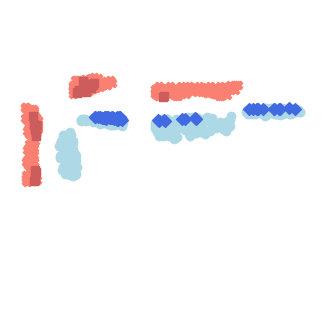
\includegraphics[width=6cm]{Battle_1.png}
      \caption{Simulation 1}
      \label{fig:Simulation}
  \centering
\end{figure}

\begin{figure}[!ht]
  \centering
      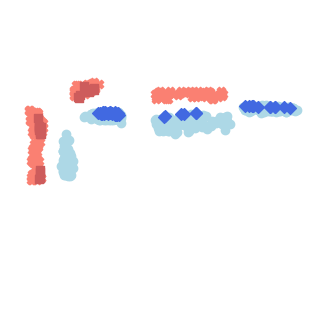
\includegraphics[width=6cm]{Battle_2.png}
      \caption{Simulation 5}
      \label{fig:Simulation}
  \centering
\end{figure}

\begin{figure}[!ht]
  \centering
      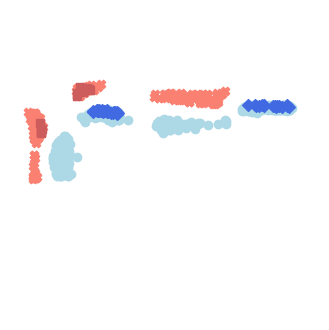
\includegraphics[width=6cm]{Battle_3.png}
      \caption{Simulation 10}
      \label{fig:Simulation}
  \centering
\end{figure}


After concluding these simulations, we can conclude that the Union overwhelmed the Confederates with their number in battle, meaning the Confederates would have been doomed one way or anther due to the overwhelming numbers of the Union. That said, if the numbers would have been more equal, it would be safe to say that the battle could have been won by either side, as showed in Figures 6, 7, and 8. In these simulations, we manipulated the number of agents per team to be equal, thus eliminating the advantage the Union had of overwhelming numbers over the Confederates. It is my conclusion, that were the numbers equal in the battle, whomever controlled the 
In these cases, the Confederate army would have overrun the Union defenses, giving way for the rest of the armies from the South to attack the northern territories, changing the course of history.

%Photo of different scenario
\begin{figure}[!ht]
  \centering
      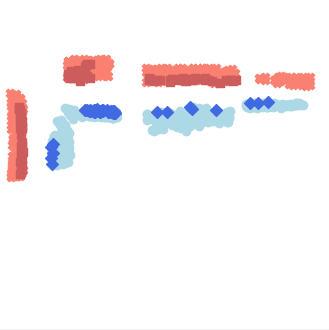
\includegraphics[width=6cm]{Equal_Battle.png}
      \caption{Equal Battle Simulation 1}
      \label{fig:Simulation}
  \centering
\end{figure}

\begin{figure}[!ht]
  \centering
      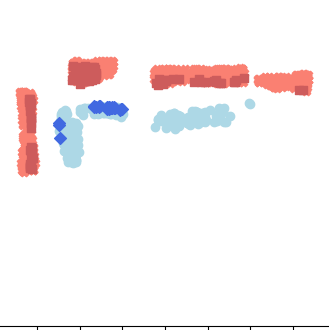
\includegraphics[width=6cm]{Equal_battle_2.png}
      \caption{Equal Battle Simulation 2}
      \label{fig:Simulation}
  \centering
\end{figure}

\begin{figure}[!ht]
  \centering
      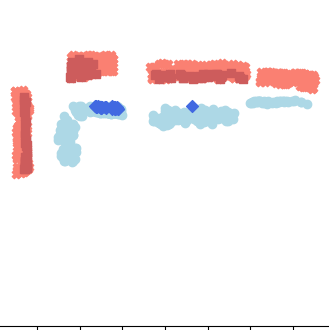
\includegraphics[width=6cm]{Equal_battle_3.png}
      \caption{Equal Battle Simulation 3}
      \label{fig:Simulation}
  \centering
\end{figure}

\section{Summary and Future work}
%%\label{}
In reexamining the Battle of Gettysburg through agent-based modeling and game theory, our study offers fresh insights into the complexities of historical decision-making. By simulating the battle dynamics, we illuminate the interplay of strategy, uncertainty, and numerical advantage that shaped the outcome. Our simulations underscore the crucial role of numbers in historical conflicts, highlighting the delicate balance between strategy and resources.

Our simulations emphasized the decisive impact of numerical superiority on battle outcomes. The Union's overwhelming numbers played a crucial role in securing victory. Moreover, when the numbers were equalized, the balance between strategy and brute force became evident, highlighting the fine line between triumph and defeat.

As for the future of this project, I would like to add more parameters to create more of a realistic simulation, as well as passing the visualization model onto a more visible engine that could create a better model.


\section*{Acknowledgements}
I want to give my thanks to my mentor, Mitchell Burdorf, as he has supported the realization of this project

%% If you have bibdatabase file and want bibtex to generate the
%% bibitems, please use
%%
\bibliographystyle{elsarticle-harv} 
\begin{thebibliography}{9}
\bibitem  Gettysburg Historic Crossroads (July 15th, 2023) \emph {https://www.gettysburgpa.gov/history/slideshows/battle-history}, Pennsylvania Gov.
\bibitem  Gettysburg (July 15th, 2023) \emph {https://www.gettysburgpa.gov/history/slideshows/battle-history}, American Battlefield Trust.
\bibitem  NashPy Documentation (July 11th, 2023) \emph{https://nashpy.readthedocs.io/en/stable/tutorial/index.html}
\end{thebibliography}
%% else use the following coding to input the bibitems directly in the
%% TeX file.

%%\begin{thebibliography}{00}

%% \bibitem[Author(year)]{label}
%% For example:

%% \bibitem[Aladro et al.(2015)]{Aladro15} Aladro, R., Martín, S., Riquelme, D., et al. 2015, \aas, 579, A101


%%\end{thebibliography}

\end{document}

\endinput
%%
